\documentclass[12pt,xcolor=table,aspectratio=169]{beamer}
\usetheme{Frankfurt}
\usecolortheme{rose}
\usepackage{amsthm}
\usepackage{amsmath}
\usepackage{bbm}
\usepackage{amsfonts}
\usepackage{amssymb}
\usepackage{graphicx}
\usepackage{hyperref}
\usepackage[flushleft]{threeparttable}
\usepackage{tabularx}
\usepackage{booktabs}
\usepackage{siunitx}
\usepackage{tikz}
\usetikzlibrary{decorations.pathreplacing,angles,quotes}

%set up course and number

\newcommand{\ClassName}{TBD}
\newcommand{\ClassNumber}{TBD}
\newcommand{\Topic}{TBD}

% Some optional colors. Change or add as you see fit.
%---------------------------------------------------
 \definecolor{ualbertagreen}{HTML}{007C41}
\definecolor{ualbertagold}{HTML}{FFDB05}

\definecolor{calloutgrey}{HTML}{D9D9D9}


%set fonts
\setbeamerfont{subtitle}{size=\large,shape=\scshape,series=\bfseries}
\setbeamerfont{title}{size=\Large,shape=\scshape,series=\bfseries}
\setbeamerfont{author}{size=\large}
\setbeamerfont{date}{size=\large}
\setbeamerfont{caption}{size=\scriptsize}


% Some optional color adjustments to Beamer. Change as you see fit.
%------------------------------------------------------------------
\setbeamercolor{frametitle}{fg=ualbertagreen,bg=white}
\setbeamercolor{title}{fg=ualbertagreen,bg=white}
\setbeamercolor{author}{fg=ualbertagreen,bg=white}
\setbeamercolor{date}{fg=ualbertagreen,bg=white}
\setbeamercolor{local structure}{fg=ualbertagreen}
\setbeamercolor{section in toc}{fg=ualbertagreen,bg=white}
% \setbeamercolor{subsection in toc}{fg=ualbertagreen,bg=white}
\setbeamercolor{footline}{fg=ualbertagreen!50, bg=white}

% definition boxes
\setbeamercolor{block title}{bg=ualbertagreen,fg=white}
\setbeamercolor{block body}{parent=normal text,use=block title,bg=calloutgrey}
%\setbeamercolor{block body}{parent=normal text,use=block title,bg=block title.bg!30!bg}


\setbeamercolor{upper separation line head}{bg=ualbertagreen}
\setbeamercolor{lower separation line head}{bg=ualbertagold}
\setbeamercolor{middle separation line head}{bg=ualbertagold}
\setbeamercolor{frametitle}{fg=ualbertagreen,bg=white}



\setbeamercolor{section in head/foot}{bg=white,fg=ualbertagreen}
\setbeamercolor{author in head/foot}{bg=white,fg=ualbertagreen}
\setbeamercolor{date in head/foot}{bg=white,,fg=ualbertagreen}
\setbeamercolor{title in head/foot}{bg=white,fg=ualbertagreen}

\setbeamercolor{headline}{bg=white,fg=ualbertagreen}




\setbeamercolor*{middle separation line head}{bg=ualbertagreen}
\setbeamercolor*{alerted text}{fg=ualbertagreen}
\setbeamercolor*{example text}{fg=black}
\setbeamercolor*{structure}{fg=black}


\let\Tiny=\tiny



\logo{
   %\ifnum\insertpagenumber>1
   \tikz [remember picture,overlay]
    \node[yshift=.3cm,xshift=1.5cm] at (current page.south west)
        %or: (current page.center)
        {\includegraphics[width=1in]{../images/UA-ASB-COLOUR.png}};
    %\fi
%\includegraphics[height=0.8cm]{../images/UA-ASB-COLOUR.png}\vspace{220pt}
}


\setbeamertemplate{title page}{%
  \vbox{}
    \vspace{.5cm}% NEW
  \begingroup
    \centering
    \begin{beamercolorbox}[sep=8pt,center]{title}
      \usebeamerfont{title}\ClassNumber: \ClassName\par%
      \usebeamerfont{title}\inserttitle\par%
     \ifx\insertsubtitle\@empty%
      \else%
        \vskip0.05em%
        {\usebeamerfont{subtitle}\usebeamercolor[fg]{subtitle}\insertsubtitle\par}%
      \fi%
    \end{beamercolorbox}%
    \begin{beamercolorbox}[sep=8pt,center]{author}
      \usebeamerfont{author}\insertauthor
    \end{beamercolorbox}
    \begin{beamercolorbox}[sep=8pt,center]{institute}
      \usebeamerfont{institute}\insertinstitute
    \end{beamercolorbox}

    \vspace{0.5cm}% NEW
    \begin{beamercolorbox}[sep=8pt,center]{date}
      \usebeamerfont{date}\insertdate
    \end{beamercolorbox}\vskip0.05em

      \endgroup
  %\vfill
}


\setbeamertemplate{frametitle}{%
    \insertframetitle\par\vskip-10pt
}



\renewcommand{\ClassName}{Business Economics, Organization and Management}
\renewcommand{\ClassNumber}{BUEC 311}

\setbeamertemplate{headline}{%
\leavevmode%
 \hbox{%
    \begin{beamercolorbox}[wd=\paperwidth,ht=5ex,dp=0ex]{white}%
    \usebeamerfont{headline}\hskip6pt\ClassNumber: \inserttitle\par%
    \insertsectionnavigationhorizontal{\paperwidth}{}{\hskip0pt plus1filll}
    \end{beamercolorbox}%
  }
}

\defbeamertemplate*{footline}{my footline}{%
    \ifnum\insertpagenumber=1
        \Tiny{%
            \hfill%
		\vspace*{1pt}%
            %\insertframenumber/\inserttotalframenumber \hspace*{0.1cm}%
            \newline%
            \color{ualbertagold}{\rule{\paperwidth}{0.4mm}}\newline%
            \color{ualbertagold}{\rule{\paperwidth}{.4mm}}%
        }
  \else%
        \Tiny{%
            \hspace{.66\paperwidth}
            %\vspace{25pt}
            \insertframenumber/\inserttotalframenumber
            \newline%
            \color{ualbertagold}{\rule{\paperwidth}{0.4mm}}\newline%
            \color{ualbertagold}{\rule{\paperwidth}{.4mm}}%
        }%
    \fi%
}


\title{Supply and Demand - The Basics}


\date{Fall 2020}

\begin{document}
\setcounter{subsection}{1}
\begin{frame}
   %\tikz [remember picture,overlay]
    %\node[yshift=-1.05cm,xshift=0cm] at (current page.north)
        %or: (current page.center)
        %\node[yshift=-0.95cm,xshift=3.5cm] at (current page.north west)
        %{\includegraphics[width=3in]{UA-ASB-COLOUR.png}};
    %    {\includegraphics[width=.4\paperwidth]{../images/UA-ASB-COLOUR.png}}; \vspace{1cm}
   \titlepage
   \vfill
\end{frame}

\section{Outline}

\frame{
	\frametitle{Outline}
	\begin{enumerate}
	\item The Supply-and-Demand Model
		\begin{itemize}
		\item Demand
		\item Supply
		\item Market Equilibrium
		\end{itemize}
	\item Using the Model
		\begin{itemize}
		\item Changing fundamentals.
		\item The effects of government intervention.
		\end{itemize}
	\item Applying the model in practice.
		\begin{itemize}
		\item When it works.
		\item When if fails.
		\end{itemize}
	\end{enumerate}
\vfill
}


\frame{
	\frametitle{Outline}
	\begin{enumerate}
	\item \alert{The Supply-and-Demand Model}
		\begin{itemize}
		\item Demand
		\item Supply
		\item Market Equilibrium
		\end{itemize}
	\item Using the Model
		\begin{itemize}
		\item Changing fundamentals.
		\item The effects of government intervention.
		\end{itemize}
	\item Applying the model in practice.
		\begin{itemize}
		\item When it works.
		\item When if fails.
		\end{itemize}
	\end{enumerate}
\vfill
}

\section{Supply and Demand}


\frame{
	\frametitle{1. The Supply-and-Demand Model}
	\begin{itemize}
	\item Supply and demand is the core of almost every economic model
	\item[]
	\item This simple model is useful for understanding many markets.
		\begin{itemize}
		\item It works particularly well in markets with many buyers and sellers.
		\end{itemize}
	\item[]
	\item Why is it useful?
		\begin{itemize}
		\item We can use it to make clear predictions about how changes in fundamentals affect
market outcomes.
        \item The limitations are easy to understand
		\end{itemize}
	\end{itemize}
}

\frame{
	\frametitle{1. The Supply-and-Demand Model: Demand}
	\begin{itemize}
	\item The first piece of the model: \textbf{Demand}
	\item[]
	\item Demand is consumer's \textit{desire} to purchase goods and services.
	\item[]
	\item What factors affect this desire? How?
	\end{itemize}
}

\frame{
	\frametitle{1. The Supply-and-Demand Model: Demand}
	\begin{itemize}
	\item While many factors can affect consumer's desire to purchase goods and services, economists
primarily focus on how a good's \textit{own price} affects the quantity demanded.
	\end{itemize}
	\bigskip
		\begin{definition}[Quantity Demanded]
		The quantity demanded is the amount of a good or service a consumer is \textit{willing} to buy
at a given price, holding other factors constant.
		\end{definition}	
}

\frame{
	\frametitle{1. The Supply-and-Demand Model: Demand}
	\begin{itemize}
	\item Empirical evidence suggests that the quantity demanded by consumers follows the \textit{Law
of Demand}.
	\end{itemize}
	
		\begin{definition}[Law of Demand]
		Consumers demand a higher quantity of a good or service when the price is lower (and a lower
quantity of when the price is higher), \textit{holding all other factors that influence the amount
consumers want to consume constant}.
		\end{definition}
		
	\begin{itemize}
	\item We can illustrate this relationship graphically using a \textit{demand curve}.
		\begin{itemize}
		\item To do so, let's use the example of gasoline demand.
		\end{itemize}
	\end{itemize}
}

\frame{
	\frametitle{1. The Supply-and-Demand Model: The Demand Curve}
	%	The demand for gasoline:
	
	\begin{figure}[t!]
	\center
	\resizebox{!}{.45\linewidth}{
\includegraphics[width=\textwidth]{../images/gas_demand.png}
}
\caption{The demand for gasoline}
\end{figure}
}


\frame{
	\frametitle{1. The Supply-and-Demand Model: The Demand Curve}
	%	The demand for gasoline:
	
	\begin{figure}[t!]
	\center
	\resizebox{!}{.45\linewidth}{
\includegraphics[width=\textwidth]{../images/gas_demand_zoom.png}
}
\caption{The demand for gasoline}
\end{figure}
}


\frame{
	\frametitle{1. The Supply-and-Demand Model: The Demand Curve}
	\begin{itemize}
	\item The demand curve provides a concise answer to the question of what happens to the quantity
demanded as price changes, holding all other factors constant.
		\begin{itemize}
		\item Here: what happens to the demand for gasoline as the price of gasoline increases or
decreases.
		\end{itemize}
	\item[]
	\item Changes in the quantity demanded in response to a price change are referred to as
\textit{movements along the demand curve}.
	\item[]
	\item Why is the demand curve downward sloping?
	\end{itemize}
}

\frame{
	\frametitle{1. The Supply-and-Demand Model: The Demand Curve}
	\begin{itemize}
	\item The demand curve tells us how a change in the price of a good or service affects the
quantity demanded.
		\begin{itemize}
		\item Change in $p$ $\implies$ \textit{movement along the demand curve}.
		\end{itemize}
	\item[]
	\item Recall that other factors also affect the quantity demanded.
		\begin{itemize}
		\item Change in these factors $\implies$ \textit{shift of the demand curve}.
		\end{itemize}
	\item[]
	\item As an example, let's consider an increase in household income. How would you expect that to change gasoline demand?
	\end{itemize}
}

\frame{
	\frametitle{1. The Supply-and-Demand Model: The Demand Curve}
		%	The demand for gasoline:
	
	\begin{figure}[t!]
	\center
	\resizebox{!}{.45\linewidth}{
\includegraphics[width=\textwidth]{../images/gas_inc.png}
}
\caption{The effects of an income increase on the demand for gasoline}
\end{figure}
}

\frame{
	\frametitle{1. The Supply-and-Demand Model: The Demand Curve}
		%	The demand for gasoline:
	
	\begin{figure}[t!]
	\center
	\resizebox{!}{.45\linewidth}{
\includegraphics[width=\textwidth]{../images/gas_inc2.png}
}
\caption{The effects of an income increase on the demand for gasoline}
\end{figure}
}


\frame{
	\frametitle{1. The Supply-and-Demand Model: The Demand Curve}
	\begin{itemize}
	\item How the demand curve shifts depends on the factor being considered.
		\begin{itemize}
		\item Income
		\item Price of substitute or compliment
		\item Tastes
		\item Government rules/regulations
		\end{itemize}
	\item[]
	\item As another example, let's consider the effects of an increase in the price tolls in the core of the city, a complement to gasoline.
	\end{itemize}
}

\frame{
	\frametitle{1. The Supply-and-Demand Model: The Demand Curve}
	%	The demand for gasoline:
	
		\begin{figure}[t!]
	\center
	\resizebox{!}{.45\linewidth}{
\includegraphics[width=\textwidth]{../images/gas_inc_comp.png}
}
\caption{The effects of an increase in the price of tolls on the demand for gasoline}
\end{figure}
}

\frame{
	\frametitle{1. The Supply-and-Demand Model: The Demand Curve}
	%	The demand for gasoline:
	
		\begin{figure}[t!]
	\center
	\resizebox{!}{.45\linewidth}{
\includegraphics[width=\textwidth]{../images/gas_inc_comp2.png}
}
\caption{The effects of an increase in the price of tolls on the demand for gasoline}
\end{figure}
}



\frame{
	\frametitle{1. The Supply-and-Demand Model: The Demand Curve}
	\begin{itemize}
	\item The demand curve gives us a precise relationship between price and quantity demanded.
	\item We can also express this same relationship mathematically using a \textit{demand function}.
	\item The demand function is given by:
		\begin{align*}
		Q = D(p,Y,X)
		\end{align*}
	where $Q$ is the quantity demanded, and $D(\cdot)$ is the demand function that depends on the price,
$p$, income, $Y$, and other factors, $X$.
	\item For simplicity, in what follows we will hold other factors ($X$) constant.
	\end{itemize}
}

\frame{
	\frametitle{1. The Supply-and-Demand Model: The Demand Function}
	\begin{itemize}
	\item Suppose that the estimated demand function for gasoline is given by:
		\begin{align*}
		Q = 13 - 2p + 0.1Y
		\end{align*}
	where $Q$ is the quantity of gasoline demanded, $p$ is the price of gasoline, and $Y$ is average
household income.
	\item[]
	\item Functional form reflects available evidence about the demand for cheesey:
		\begin{itemize}
		\item $p$ is negative.
		\item $Y$ is positive.
		\item Constant term ($13$) reflects all other factors.
		\end{itemize}
	\end{itemize}
}

\frame{
	\frametitle{1. The Supply-and-Demand Model: The Demand Function}
	\begin{itemize}
	\item We can obtain the demand curve for gasoline by substituting for income, $Y$.
	\item[]
	\item Suppose average household income is \$10,000. Then the demand for gasoline is given by:
		\begin{align*}
		Q &= 13 - 2p + 0.1(10)\\
			&= 14 - 2p
		\end{align*}
	\item With some algebra we can obtain the \textit{inverse demand curve}:
		\begin{align*}
		p = 7 -\frac{1}{2}Q
		\end{align*}
	\item This is the same relationship depicted on the next slide.
	\end{itemize}
}

\frame{
	\frametitle{1. The Supply-and-Demand Model: The Demand Function}
	%	The demand for gasoline:
	
	\begin{figure}[t!]
	\center
	\resizebox{!}{.35\linewidth}{

	\begin{tikzpicture}
	% Draw axes
	%Y
	\draw[->] (0,0) -- (0,10) ;
	\draw[] (0,8) -- node[rotate=90, above=30pt] {\textbf{$p$, \$ per kg}} (0,8);
	%X
	\draw[->] (0,0) -- (15,0);
	\draw[] (14,0) -- node[below=30pt] {\textbf{$Q$, millions of kg per year}} (14,0);

	% Plot demand curve:
	% Curve given by: Q = 13 - 2p + 0.1Y
	% Assume Y= 10
	% Inverse demand: p = 7-0.5*Q
	\draw[color=black, thick, domain=0:14] plot (\x,{7-0.5*\x});
	\node at (6,6) [below] {Demand Curve for Gasoline, $D$};

	%Plot illustrative lines
	\draw[dashed] (0,5) -- (4,5) -- (4,0);
	\draw[dashed] (0,3) -- (8,3) -- (8,0);
	\draw[dashed] (0,1) -- (12,1) -- (12,0);

	%Add axes labels
	%Origin%
	\node at (0,0) [left] {{0}};
	%Y Axis
	\node at (0,7) [left] {{7.00}};
	\node at (0,5) [left] {{5.00}};
	\node at (0,3) [left] {{3.00}};
	\node at (0,1) [left] {{1.00}};
	%X Axis
	\node at (4,0) [below] {{4}};
	\node at (8,0) [below] {{8}};
	\node at (12,0) [below] {{12}};
	\node at (14,0) [below] {{14}};

\end{tikzpicture}
}
\caption{The demand for gasoline}
\end{figure}
}

\frame{
	\frametitle{1. The Supply-and-Demand Model: The Demand Function}
	\begin{itemize}
	\item The demand function is useful because it allows us to think precisely about how the
quantity demanded will respond to a change in price, holding income (and all other factors) fixed.
	\item[]
	\item To see this, let $p_{1}$ denote the initial price, and $p_{2}$ denote the new price. Then
the quantity demanded at $p_{1}$ is $Q_{1}=D(p_{1})$, the quantity demanded at $p_{2}$ is
$Q_{2}=D(p_{2})$, and the change in quantity demanded as price goes from $p_{1}$ to $p_{2}$ is
$\Delta Q = Q_{2}-Q_{1} = D(p_{2})-D(p_{1})$.
	\item[]
	\item In our gasoline example, if the price changes from $p_{1}$ to $p_{2}$, the change in
quantity demanded is given by:
		\begin{align*}
		\Delta Q &= D(p_{2})-D(p_{1}) = [14-2p_{2}]-[14-2p_{1}]\\
			& = -2[p_{2}-p_{1}] = -2 \Delta p
		\end{align*}
	\end{itemize}	
}

\frame{
	\frametitle{1. The Supply-and-Demand Model: Determining Market Demand}
	\begin{itemize}
	\item In many cases we might have an estimate of the demand from all consumers in a market, but
in some scenarios, we may only know the demands of individual consumers or groups of consumers.
	\item[]
	\item In these cases, we need to add up the demand from each consumer (or group).
	\item[]
	\item Key point: Total quantity demanded \textit{at a given price} is equal to the sum of
individual consumer demands at that price.
	\end{itemize}
}

\frame{
	\frametitle{1. The Supply-and-Demand Model: Determining Market Demand}
	\begin{itemize}
	\item As an example, suppose there are two people in the market for gasoline. They both have
demand functions given by:
		\begin{align*}
		Q = 14-2p
		\end{align*}
		What is the market demand for gasoline in this case?
	\end{itemize}
}

\frame{
	\frametitle{1. The Supply-and-Demand Model: Supply}
	\begin{itemize}
	\item The second piece of the model: \textbf{Supply}
	\item[]
	\item Supply is producers' willingness to sell goods and services.
	\item[]
	\item What factors affect this willingness? How?
	\end{itemize}	
}

\frame{
	\frametitle{1. The Supply-and-Demand Model: Supply}
	\begin{itemize}
	\item As with demand, economist focus on how the \textit{price} of a good or service affects the
quantity supplied.
	\end{itemize}
	\begin{definition}[Quantity Supplied]
	The amount of a good or service that producers \textit{want} to sell at a given price,
\textit{holding other factors that influence supply decisions constant}.
	\end{definition}
}

\frame{
	\frametitle{1. The Supply-and-Demand Model: Supply}
	\begin{itemize}
	\item Is there a Law of Supply?
	\item[]
	\item We can illustrate the relationship between the price of a good or service and the quantity
producers want to sell via a \textit{supply curve}.
	\end{itemize}
}

\frame{
	\frametitle{1. The Supply-and-Demand Model: The Supply Curve}
	%	The demand for gasoline:
	
	\begin{figure}[t!]
	\center
	\resizebox{!}{.35\linewidth}{

	\begin{tikzpicture}
	% Draw axes
	%Y
	\draw[->] (0,0) -- (0,10) ;
	\draw[] (0,8) -- node[rotate=90, above=30pt] {\textbf{$p$, \$ per kg}} (0,8);
	%X
	\draw[->] (0,0) -- (15,0);
	\draw[] (14,0) -- node[below=30pt] {\textbf{$Q$, millions of kg per year}} (14,0);

	% Plot supply curve:
	% Curve given by: Q = 1 + 2p - 0.5p_{y}
	% Assume p_{y}= 2
	% Inverse demand: p = 0.5*Q
	\draw[color=black, thick, domain=0:14] plot (\x,{0.5*\x});
	\node at (8,7) [right] {Supply Curve for Gasoline, $S$};

	%Plot illustrative lines
	\draw[dashed] (0,5) -- (10,5) -- (10,0);
	\draw[dashed] (0,3) -- (6,3) -- (6,0);
	\draw[dashed] (0,1) -- (2,1) -- (2,0);

	%Add axes labels
	%Origin%
	\node at (0,0) [left] {{0}};
	%Y Axis
%	\node at (0,7) [left] {{7.00}};
	\node at (0,5) [left] {{5.00}};
	\node at (0,3) [left] {{3.00}};
	\node at (0,1) [left] {{1.00}};
	%X Axis
	\node at (2,0) [below] {{2}};
	\node at (6,0) [below] {{6}};
	\node at (10,0) [below] {{10}};
%	\node at (14,0) [below] {{14}};

\end{tikzpicture}
}
\caption{The supply of gasoline}
\end{figure}
}

\frame{
	\frametitle{1. The Supply-and-Demand Model: The Supply Curve}
	\begin{itemize}
	\item The supply curve provides us an answer to the question of what happens to the quantity
supplied as price changes, holding all other factors fixed.
		\begin{itemize}
		\item Here: what happens to the supply of gasoline as the price of gasoline increases or
decreases.
		\end{itemize}
	\item[]
	\item Changes in the quantity supplied in response to a price change are referred to as
\textit{movements along the supply curve}.
	\item[]
	\item Do supply curves always need to slope upward?
	\end{itemize}
}

\frame{
	\frametitle{1. The Supply-and-Demand Model: The Supply Curve}
	\begin{itemize}
	\item The supply curve tells us how a change in the price of a good or service affects the
quantity supplied.
		\begin{itemize}
		\item Change in $p$ $\implies$ \textit{movement along the supply curve}.
		\end{itemize}
	\item[]
	\item Recall that other factors also affect the quantity supplied.
		\begin{itemize}
		\item Change in these factors $\implies$ shift of the supply curve.
		\end{itemize}
	\item[]
	\item As an example, let's suppose that the price of an alternative product, yoghurt, increases
in price from \$2.00 per kg to \$4.00 per kg.
	\end{itemize}
}

\frame{
	\frametitle{1. The Supply-and-Demand Model: The Supply Curve}
	%	The demand for gasoline:
	
	\begin{figure}[t!]
	\center
	\resizebox{!}{.35\linewidth}{

	\begin{tikzpicture}
	% Draw axes
	%Y
	\draw[->] (0,0) -- (0,10) ;
	\draw[] (0,8) -- node[rotate=90, above=30pt] {\textbf{$p$, \$ per kg}} (0,8);
	%X
	\draw[->] (0,0) -- (15,0);
	\draw[] (14,0) -- node[below=30pt] {\textbf{$Q$, millions of kg per year}} (14,0);

	% Plot supply curve:
	% Curve given by: Q = 1 + 2p - 0.5p_{y}
	% Assume p_{y}= 2
	% Inverse demand: p = 0.5*Q
	\draw[color=black, thick, domain=0:14] plot (\x,{0.5*\x});
	\node at (11,5) [right] {Original Supply Curve, $S^{1}$};
	\draw[->] (13,5.5) -- (12.5,6);

	% Now p_{y} = 4, so Q = -1 + 2p
	% Inverse demand: p =.5+ 0.5*Q
	\draw[color=red, thick, domain=0:14] plot (\x,{0.5+0.5*\x});
	\node at (7,7) [right] {New Supply Curve, $S^{2}$};
	\draw[->] (9,6.5) -- (10,6);

	%Plot illustrative lines
	\draw[dashed] (0,3) -- (6,3) -- (6,0);
	\draw[dashed] (5,3) -- (5,0);

	%Add axes labels
	%Origin%
	\node at (0,0) [left] {{0}};
	%Y Axis
	\node at (0,3) [left] {{3.00}};
	%X Axis
	\node at (5,0) [below] {{5}};
	\node at (6,0) [below] {{6}};

\end{tikzpicture}
}
\caption{The effect of a yogurt price increase on the supply of gasoline}
\end{figure}
}

\frame{
	\frametitle{1. The Supply-and-Demand Model: The Supply Curve}
	\begin{itemize}
	\item How the supply curve shifts depends on the factor being considered.
		\begin{itemize}
		\item Prices.
		\item Production costs.
		\item Technological change.
		\item Government regulation.
		\end{itemize}
	\item[]
	\item As another example, let's consider the effects of a decrease in the price of milk.
	\end{itemize}

}

\frame{
	\frametitle{1. The Supply-and-Demand Model: The Supply Curve}
	%	The demand for gasoline:
	
	\begin{figure}[t!]
	\center
	\resizebox{!}{.35\linewidth}{

	\begin{tikzpicture}
	% Draw axes
	%Y
	\draw[->] (0,0) -- (0,10) ;
	\draw[] (0,8) -- node[rotate=90, above=30pt] {\textbf{$p$, \$ per kg}} (0,8);
	%X
	\draw[->] (0,0) -- (15,0);
	\draw[] (14,0) -- node[below=30pt] {\textbf{$Q$, millions of kg per year}} (14,0);

	% Plot supply curve:
	% Curve given by: Q = 1 + 2p - 0.5p_{y}
	% Assume p_{y}= 2
	% Inverse demand: p = 0.5*Q
	\draw[color=black, thick, domain=0:14] plot (\x,{0.5*\x});
	\node at (7,6) [right] {Original Supply Curve, $S^{1}$};
	\draw[->] (9,5.5) -- (10,5.25);

	% Now Q = 2+ 2p
	% Inverse demand: p =-1+ 0.5*Q
	\draw[color=red, thick, domain=2:14] plot (\x,{-1+0.5*\x});
	\node at (11,4) [right] {New Supply Curve, $S^{2}$};
	\draw[->] (13,4.5) -- (12.5,5);
	
	%Plot illustrative lines
	\draw[dashed] (0,3) -- (6,3) -- (6,0);
	\draw[dashed] (6,3) -- (8,3) -- (8,0);

	%Add axes labels
	%Origin%
	\node at (0,0) [left] {{0}};
	%Y Axis
	\node at (0,3) [left] {{3.00}};
	%X Axis
	\node at (6,0) [below] {{6}};
	\node at (8,0) [below] {{8}};

\end{tikzpicture}
}
\caption{The effect of a decrease in the price of milk on the supply of gasoline}
\end{figure}
}

\frame{
	\frametitle{The Supply-and-Demand Model: The Supply Curve}
	\begin{itemize}
	\item The supply curve displays a precise relationship between price and quantity supplied.
	\item[]
	\item We can also express this same relationship mathematically using a \textit{supply function}.
	\item[]
	\item The supply function is given by:
		\begin{align*}
		Q = S(p,p_{y},X)
		\end{align*}
		where $Q$ is the quantity supplied, and $S(-)$ is the supply function that depends on the
price, $p$, the price of other possible outputs $p_{y}$, and other factors, $X$.
	\item[]
	\item For simplicity, in what follows, we will hold other factors ($X$) constant.
	\end{itemize}
}

\frame{
	\frametitle{The Supply-and-Demand Model: The Supply Function}
	\begin{itemize}
	\item Suppose that the estimated supply function for gasoline is given by:
		\begin{align*}
		Q =  1 + 2p - 0.5p_{y}
		\end{align*}
		where $Q$ is the quantity of gasoline supplied, $p$ is the price of gasoline, and $p_{y}$ is
the price of alternative outputs (yoghurt).
	\item[]
	\item Functional form reflects available evidence about the supply of gasoline:
		\begin{itemize}
		\item $p$ is positive.
		\item $p_{y}$ is negative.
		\item The constant term (1) reflects all other factors.
		\end{itemize}
	\end{itemize}
}

\frame{
	\frametitle{The Supply-and-Demand Model: The Supply Function}
	\begin{itemize}
	\item We can obtain the supply curve by substituting for $p_{y}$.
	\item[]
	\item Suppose the price of yoghurt is \$2.00. Then the supply of gasoline is given by:
		\begin{align*}
		Q & = 1 + 2p - 0.5(2)\\
		 & = 2 p
		\end{align*}
	\item Rearranging we can obtain the \textit{inverse supply curve}.
		\begin{align*}
		p= \frac{1}{2} Q
		\end{align*}
	\item This is the same relationship depicted on the next slide.
	\end{itemize}
}

\frame{
	\frametitle{1. The Supply-and-Demand Model: The Supply Function}
	%	The demand for gasoline:
	
	\begin{figure}[t!]
	\center
	\resizebox{!}{.35\linewidth}{

	\begin{tikzpicture}
	% Draw axes
	%Y
	\draw[->] (0,0) -- (0,10) ;
	\draw[] (0,8) -- node[rotate=90, above=30pt] {\textbf{$p$, \$ per kg}} (0,8);
	%X
	\draw[->] (0,0) -- (15,0);
	\draw[] (14,0) -- node[below=30pt] {\textbf{$Q$, millions of kg per year}} (14,0);

	% Plot supply curve:
	% Curve given by: Q = 1 + 2p - 0.5p_{y}
	% Assume p_{y}= 2
	% Inverse demand: p = 0.5*Q
	\draw[color=black, thick, domain=0:14] plot (\x,{0.5*\x});
	\node at (8,7) [right] {Supply Curve for Gasoline, $S$};

	%Plot illustrative lines
	\draw[dashed] (0,5) -- (10,5) -- (10,0);
	\draw[dashed] (0,3) -- (6,3) -- (6,0);
	\draw[dashed] (0,1) -- (2,1) -- (2,0);

	%Add axes labels
	%Origin%
	\node at (0,0) [left] {{0}};
	%Y Axis
%	\node at (0,7) [left] {{7.00}};
	\node at (0,5) [left] {{5.00}};
	\node at (0,3) [left] {{3.00}};
	\node at (0,1) [left] {{1.00}};
	%X Axis
	\node at (2,0) [below] {{2}};
	\node at (6,0) [below] {{6}};
	\node at (10,0) [below] {{10}};
%	\node at (14,0) [below] {{14}};

\end{tikzpicture}
}
\caption{The supply of gasoline}
\end{figure}
}

\frame{
	\frametitle{1. The Supply-and-Demand Model: The Supply Function}
	\begin{itemize}
	\item The supply function allows us to think precisely about how price changes affect the
quantity supplied, holding all other factors fixed.
	\item[]
	\item To see this let $p_{1}$ denote the initial price, and $p_{2}$ denote the new price. Then
the quantity supplied at $p_{1}$ is $Q_{1} = S(p_{1})$, the quantity supplied  at $p_{2}$ is $Q_{2} =
S(p_{2})$, and the change in quantity supplied as price goes from $p_{1}$ to $p_{2}$ is $\Delta Q =
Q_{2}-Q_{1} = S(p_{2})-S(p_{1})$.
	\item[]
	\item In our gasoline example, if the price changes from $p_{1}$ to $p_{2}$, the change in
quantity supplied is given by:
		\begin{align*}
		\Delta Q &= S(p_{2}) - S(p_{1}) = [2 p_{2}]- [2 p_{1}]\\
			& = 2 [p_{2}-p_{1}] = 2 \Delta p
		\end{align*}
	\end{itemize}
}

\frame{
	\frametitle{1. The Supply-and-Demand Model: Determining Market Supply}
	\begin{itemize}
	\item In some cases, we may not have an estimate of total market supply, but rather estimates of
the supply curves of each producer in the market.
	\item[]
	\item To obtain total market supply, we need to add up the supply from each producer.
	\end{itemize}
}	

\frame{
	\frametitle{1. The Supply-and-Demand Model: Determining Market Supply}
	\begin{itemize}
	\item As an example, suppose there are 3 producers in the market for gasoline. They both have
supply functions given by:
		\begin{align*}
		Q = 2p
		\end{align*}
		what is the market supply of gasoline in this case?
	\end{itemize}
}

\frame{
	\frametitle{1. The Supply-and-Demand Model: Market Equilibrium}
	\begin{itemize}
	\item Once we know supply and demand in the market, we can determine the \textit{market
equilibrium}.
	\end{itemize}
	\begin{definition}[Market Equilibrium]
	The market is in equilibrium when all market participants are able to buy or sell as much as they
want; no participant wants to change its behaviour given what other market participants are doing.
	\end{definition}
}

\frame{
	\frametitle{1. The Supply-and-Demand Model: Market Equilibrium}
	\begin{itemize}
	\item How can we determine the market equilibrium from the supply and demand curves?
	\end{itemize}
}

\frame{
	\frametitle{1. The Supply-and-Demand Model: Market Equilibrium}
	%	The demand for gasoline:
	
	\begin{figure}[t!]
	\center
	\resizebox{!}{.35\linewidth}{

	\begin{tikzpicture}
	% Draw axes
	%Y
	\draw[->] (0,0) -- (0,10) ;
	\draw[] (0,8) -- node[rotate=90, above=30pt] {\textbf{$p$, \$ per kg}} (0,8);
	%X
	\draw[->] (0,0) -- (15,0);
	\draw[] (14,0) -- node[below=30pt] {\textbf{$Q$, millions of kg per year}} (14,0);

	% Plot demand curve:
	% Curve given by: Q = 13 - 2p + 0.1Y
	% Assume Y= 10
	% Inverse demand: p = 7-0.5*Q
	\draw[color=blue, thick, domain=0:14] plot (\x,{7-0.5*\x});
	\node at (5.5,7.25) [left] {Demand Curve for Gasoline, $D$};

	% Plot supply curve:
	% Curve given by: Q = 1 + 2p - 0.5p_{y}
	% Assume p_{y}= 2
	% Inverse demand: p = 0.5*Q
	\draw[color=red, thick, domain=0:14] plot (\x,{0.5*\x});
	\node at (8,7) [right] {Supply Curve for Gasoline, $S$};

	%Plot illustrative lines
	\draw[dashed] (0,3.5) -- (7,3.5) -- (7,0);

	%Add axes labels
	%Origin%
	\node at (0,0) [left] {{0}};
	%Y Axis
	\node at (0,3.5) [left] {{3.50}};
	%X Axis
	\node at (7,0) [below] {{7}};


\end{tikzpicture}
}
\caption{Equilibrium in the market for gasoline}
\end{figure}
}

\frame{
	\frametitle{1. The Supply-and-Demand Model: Market Equilibrium}
	\begin{definition}[Equilibrium Price]
	The equilibrium price is the $p$ at which consumers can by as much as they want, and sellers can
sell as much as they want.
	\end{definition}
	
	\begin{definition}[Equilibrium Quantity]
	The equilibrium quantity is the $q$ such that the quantity demanded equals the quantity supplied.
	\end{definition}
}

\frame{
	\frametitle{1. The Supply-and-Demand Model: Market Equilibrium}
	\begin{itemize}
	\item We can also solve for the market equilibrium analytically using algebra. Recall:
		\begin{align*}
		Q_{D} = 14 - 2p \quad \text{and} \quad Q_{S} = 2p
		\end{align*}
	\item In equilibrium $Q_{D}=Q_{S}$. Substituting yields:
		\begin{align*}
		14-2p &= 2p\\
		4p &=14 \\
		p &= 3.5
		\end{align*}
	\item Substituting in the equilibrium price into $Q_{D}$ or $Q_{S}$ yields the equilibrium
quantity of 7.
	\end{itemize}
}

\frame{
	\frametitle{1. The Supply-and-Demand Model: Market Equilibrium}
	\begin{itemize}
	\item Why must $Q_{D}=Q_{S}$ in a market equilibrium?
	\end{itemize}
}

\frame{
	\frametitle{1. The Supply-and-Demand Model: Market Equilibrium}
	%	The demand for gasoline:
	
	\begin{figure}[t!]
	\center
	\resizebox{!}{.35\linewidth}{

	\begin{tikzpicture}
	% Draw axes
	%Y
	\draw[->] (0,0) -- (0,10) ;
	\draw[] (0,8) -- node[rotate=90, above=30pt] {\textbf{$p$, \$ per kg}} (0,8);
	%X
	\draw[->] (0,0) -- (15,0);
	\draw[] (14,0) -- node[below=30pt] {\textbf{$Q$, millions of kg per year}} (14,0);

	% Plot demand curve:
	% Curve given by: Q = 13 - 2p + 0.1Y
	% Assume Y= 10
	% Inverse demand: p = 7-0.5*Q
	\draw[color=blue, thick, domain=0:14] plot (\x,{7-0.5*\x});
	\node at (3.5,7.25) [left] {Demand Curve, $D$};

	% Plot supply curve:
	% Curve given by: Q = 1 + 2p - 0.5p_{y}
	% Assume p_{y}= 2
	% Inverse demand: p = 0.5*Q
	\draw[color=red, thick, domain=0:14] plot (\x,{0.5*\x});
	\node at (10,7) [right] {Supply Curve, $S$};

	%Plot illustrative lines
	\draw[dashed] (0,5) -- (10,5) -- (10,0);
	\draw[dashed] (4,5) -- (4,0);

	%Add axes labels
	%Origin%
	\node at (0,0) [left] {{0}};
	%Y Axis
	\node at (0,5) [left] {{5.00}};
	%X Axis
	\node at (4,0) [below] {{$Q_{D}=4$}};
	\node at (10,0) [below] {{$Q_{S}=10$}};
	
\end{tikzpicture}
}
\caption{Excess Supply}
\end{figure}
}

\frame{
	\frametitle{1. The Supply-and-Demand Model: Market Equilibrium}
	%	The demand for gasoline:
	
	\begin{figure}[t!]
	\center
	\resizebox{!}{.35\linewidth}{

	\begin{tikzpicture}
	% Draw axes
	%Y
	\draw[->] (0,0) -- (0,10) ;
	\draw[] (0,8) -- node[rotate=90, above=30pt] {\textbf{$p$, \$ per kg}} (0,8);
	%X
	\draw[->] (0,0) -- (15,0);
	\draw[] (14,0) -- node[below=30pt] {\textbf{$Q$, millions of kg per year}} (14,0);

	% Plot demand curve:
	% Curve given by: Q = 13 - 2p + 0.1Y
	% Assume Y= 10
	% Inverse demand: p = 7-0.5*Q
	\draw[color=blue, thick, domain=0:14] plot (\x,{7-0.5*\x});
	\node at (3.5,7.25) [left] {Demand Curve, $D$};

	% Plot supply curve:
	% Curve given by: Q = 1 + 2p - 0.5p_{y}
	% Assume p_{y}= 2
	% Inverse demand: p = 0.5*Q
	\draw[color=red, thick, domain=0:14] plot (\x,{0.5*\x});
	\node at (10,7) [right] {Supply Curve, $S$};

	%Plot illustrative lines
	\draw[dashed] (0,2) -- (10,2) -- (10,0);
	\draw[dashed] (4,2) -- (4,0);

	%Add axes labels
	%Origin%
	\node at (0,0) [left] {{0}};
	%Y Axis
	\node at (0,2) [left] {{2.00}};
	%X Axis
	\node at (4,0) [below] {{$Q_{S}=4$}};
	\node at (10,0) [below] {{$Q_{D}=10$}};
	
\end{tikzpicture}
}
\caption{Excess Demand}
\end{figure}
}

\frame{
	\frametitle{Outline}
	\begin{enumerate}
%	\item Big Government Gasoline
%	\item[]
	\item The Supply-and-Demand Model
		\begin{itemize}
		\item Demand
		\item Supply
		\item Market Equilibrium
		\end{itemize}
	\item[]
	\item \alert{Using the Model}
		\begin{itemize}
		\item Changing fundamentals.
		\item The effects of government intervention.
		\end{itemize}
	\item[]
	\item Applying the model in practice.
		\begin{itemize}
		\item When it works.
		\item When if fails.
		\end{itemize}
	\end{enumerate}
}

\section{Using the Model}

\frame{
	\frametitle{2. Using the Model}
	\begin{itemize}
	\item The supply-and-demand model tells us the price and quantity that will \textit{clear the
market} holding all other factors fixed.
	\item[]
	\item Changes in these other factors will change the market equilibrium by shifting the supply
and demand curves (or both!).
	\item[]
	\item We can use the model to precisely predict how changes in these other factors will alter the
market equilibrium.
	\item[]
	\item We will consider two sets of factors:
		\begin{enumerate}
		\item ``Market Fundamentals.''
		\item Government intervention.
		\end{enumerate}
	\end{itemize}
}

\frame{
	\frametitle{2. Using the Model: Shifting Demand}
	\begin{itemize}
	\item We will start by considering the effects of an increase in annual household income.
	\item[]
	\item Specifically, suppose that household income increases from \$10,000 to \$20,000.
	\item[]
	\item How does this affect equilibrium price and quantity?
	\end{itemize}
}

\frame{
	\frametitle{2. Using the Model: Shifting Demand}
	%	The demand for gasoline:
	
	\begin{figure}[t!]
	\center
	\resizebox{!}{.35\linewidth}{

	\begin{tikzpicture}
	% Draw axes
	%Y
	\draw[->] (0,0) -- (0,10) ;
	\draw[] (0,8) -- node[rotate=90, above=30pt] {\textbf{$p$, \$ per kg}} (0,8);
	%X
	\draw[->] (0,0) -- (15,0);
	\draw[] (14,0) -- node[below=30pt] {\textbf{$Q$, millions of kg per year}} (14,0);

	% Plot demand curve:
	% Curve given by: Q = 13 - 2p + 0.1Y
	% Assume Y= 10
	% Inverse demand: p = 7-0.5*Q
	\draw[color=blue, thick, domain=0:14] plot (\x,{7-0.5*\x});
	\node at (1,6.25) [left] {$D^{1}$};
	% Assume Y = 20
	% Inverse demand: p = 7.5-0.5*Q
	\draw[color=blue, thick, dashed, domain=0:14] plot (\x,{7.5-0.5*\x});
	\node at (1,7.75) [left] {$D^{2}$};

	% Plot supply curve:
	% Curve given by: Q = 1 + 2p - 0.5p_{y}
	% Assume p_{y}= 2
	% Inverse demand: p = 0.5*Q
	\draw[color=red, thick, domain=0:14] plot (\x,{0.5*\x});
	\node at (13.5,7.5) [right] {$S$};

	%Plot illustrative lines
	% Original Equilibrium
	\draw[dashed] (0,3.5) -- (7,3.5) -- (7,0);
	% New Equilibrium
	\draw[dashed] (0,3.75) -- (7.5,3.75) -- (7.5,0);

	%Add axes labels
	%Origin%
	\node at (0,0) [left] {{0}};
	%Y Axis
	\node at (0,3.45) [left] {{3.50}};
	\node at (0,3.85) [left] {{3.75}};
	%X Axis
	\node at (7,0) [below] {{7}};
	\node at (7.5,0) [below] {{7.5}};

\end{tikzpicture}
}
\caption{The effects of an increase in income}
\end{figure}
}

\frame{
	\frametitle{2. Using the Model: Shifting Demand}
	\begin{itemize}
	\item The increase in income shifts the demand curve to the right (from $D^{1}$ to $D^{2}$).
	\item[]
	\item This results in a \textit{movement along the supply curve}.
	\item[]
	\item Why?
	\end{itemize}
}

\frame{
	\frametitle{2. Using the Model: Shifting Demand}
	%	The demand for gasoline:
	
	\begin{figure}[t!]
	\center
	\resizebox{!}{.35\linewidth}{

	\begin{tikzpicture}
	% Draw axes
	%Y
	\draw[->] (0,0) -- (0,10) ;
	\draw[] (0,8) -- node[rotate=90, above=30pt] {\textbf{$p$, \$ per kg}} (0,8);
	%X
	\draw[->] (0,0) -- (15,0);
	\draw[] (14,0) -- node[below=30pt] {\textbf{$Q$, millions of kg per year}} (14,0);

	% Plot demand curve:
	% Curve given by: Q = 13 - 2p + 0.1Y
	% Assume Y= 10
	% Inverse demand: p = 7-0.5*Q
	\draw[color=blue, thick, domain=0:14] plot (\x,{7-0.5*\x});
	\node at (1,6.25) [left] {$D^{1}$};
	% Assume Y = 20
	% Inverse demand: p = 7.5-0.5*Q
	\draw[color=blue, thick, dashed, domain=0:14] plot (\x,{7.5-0.5*\x});
	\node at (1,7.75) [left] {$D^{2}$};

	% Plot supply curve:
	% Curve given by: Q = 1 + 2p - 0.5p_{y}
	% Assume p_{y}= 2
	% Inverse demand: p = 0.5*Q
	\draw[color=red, thick, domain=0:14] plot (\x,{0.5*\x});
	\node at (13.5,7.5) [right] {$S$};

	%Plot illustrative lines
	% Original Equilibrium
	\draw[dashed] (0,3.5) -- (7,3.5) -- (7,0);
	% New Equilibrium
	\draw[dashed] (0,3.75) -- (7.5,3.75) -- (7.5,0);
	% Excess Demand
	\draw[dashed] (7,3.5) -- (8,3.5) -- (8,0);

	%Add axes labels
	%Origin%
	\node at (0,0) [left] {{0}};
	%Y Axis
	\node at (0,3.45) [left] {{3.50}};
%	\node at (0,3.85) [left] {{3.75}};
	%X Axis
	\node at (7,0) [below] {{7}};
%	\node at (7.5,0) [below] {{7.5}};
	\node at (8,0) [below] {{8}};

\end{tikzpicture}
}
\caption{The effects of an increase in income}
\end{figure}
}

\frame{
	\frametitle{2. Using the Model: Shifting Demand}
	\begin{itemize}
	\item We can also determine the effect of an income increase using algebra. Recall:
		\begin{align*}
		Q_{d} & = 13 - 2p + 0.1 Y\\
		Q_{s} & = 2 p
		\end{align*}
	\item \underline{Step 1:} Solve for the initial equilibrium with $Y=10$.
		\begin{align*}
		Q_{d} = Q_{s} & \implies 13- 2p + 0.1(10) = 2p \\
					& \implies p = 3.5 \text{ and } Q = 7.
		\end{align*}
	\item \underline{Step 2:} Solve for the new equilibrium with $Y=20$.
		\begin{align*}
		Q_{d} = Q_{s} & \implies 13- 2p + 0.1(20) = 2p \\
					& \implies p = 3.75 \text{ and } Q = 7.5.
		\end{align*}
	\end{itemize}
}

\frame{
	\frametitle{2. Using the Model: Shifting Supply}
	\begin{itemize}
	\item Suppose instead that the price of yoghurt increase from \$2.00 to \$4.00.
	\item[]
	\item How does this affect equilibrium price and quantity?
	\end{itemize}
}

\frame{
	\frametitle{2. Using the Model: Shifting Supply}
	%	The demand for gasoline:
	
	\begin{figure}[t!]
	\center
	\resizebox{!}{.35\linewidth}{

	\begin{tikzpicture}
	% Draw axes
	%Y
	\draw[->] (0,0) -- (0,10) ;
	\draw[] (0,8) -- node[rotate=90, above=30pt] {\textbf{$p$, \$ per kg}} (0,8);
	%X
	\draw[->] (0,0) -- (15,0);
	\draw[] (14,0) -- node[below=30pt] {\textbf{$Q$, millions of kg per year}} (14,0);

	% Plot demand curve:
	% Curve given by: Q = 13 - 2p + 0.1Y
	% Assume Y= 10
	% Inverse demand: p = 7-0.5*Q
	\draw[color=blue, thick, domain=0:14] plot (\x,{7-0.5*\x});
	\node at (1,7.25) [left] {$D$};

	% Plot supply curve:
	% Curve given by: Q = 1 + 2p - 0.5p_{y}
	% Assume p_{y}= 2
	% Inverse supply: p = 0.5*Q
	\draw[color=red, thick, domain=0:14] plot (\x,{0.5*\x});
	\node at (13.5,6.5) [right] {$S^{1}$};
	
	% Assume p_{y}=4
	% Inverse supply: p = 0.5 + 0.5*Q
	\draw[color=red, thick, dashed, domain=0:14] plot (\x,{0.5+0.5*\x});
	\node at (13.5,7.75) [right] {$S^{2}$};

	%Plot illustrative lines
	% Original Equilibrium
	\draw[dashed] (0,3.5) -- (7,3.5) -- (7,0);
	% New Equilibrium
	\draw[dashed] (0,3.75) -- (6.5,3.75) -- (6.5,0);

	%Add axes labels
	%Origin%
	\node at (0,0) [left] {{0}};
	%Y Axis
	\node at (0,3.45) [left] {{3.50}};
	\node at (0,3.85) [left] {{3.75}};
	%X Axis
	\node at (7,0) [below] {{7}};
	\node at (6.5,0) [below] {{6.5}};

\end{tikzpicture}
}
\caption{The effects of an increase in the price of yoghurt}
\end{figure}
}

\frame{
	\frametitle{2. Using the Model: Shifting Supply}
	\begin{itemize}
	\item The increase in the price of yoghurt shifts the supply cure to the left (from $S^{1}$ to
$S^{2}$).
	\item[]
	\item This results in a \textit{movement along the demand curve}.
	\item[]
	\item Why?
	\end{itemize}
}

\frame{
	\frametitle{2. Using the Model: Shifting Supply}
	%	The demand for gasoline:
	
	\begin{figure}[t!]
	\center
	\resizebox{!}{.35\linewidth}{

	\begin{tikzpicture}
	% Draw axes
	%Y
	\draw[->] (0,0) -- (0,10) ;
	\draw[] (0,8) -- node[rotate=90, above=30pt] {\textbf{$p$, \$ per kg}} (0,8);
	%X
	\draw[->] (0,0) -- (15,0);
	\draw[] (14,0) -- node[below=30pt] {\textbf{$Q$, millions of kg per year}} (14,0);

	% Plot demand curve:
	% Curve given by: Q = 13 - 2p + 0.1Y
	% Assume Y= 10
	% Inverse demand: p = 7-0.5*Q
	\draw[color=blue, thick, domain=0:14] plot (\x,{7-0.5*\x});
	\node at (1,7.25) [left] {$D$};

	% Plot supply curve:
	% Curve given by: Q = 1 + 2p - 0.5p_{y}
	% Assume p_{y}= 2
	% Inverse supply: p = 0.5*Q
	\draw[color=red, thick, domain=0:14] plot (\x,{0.5*\x});
	\node at (13.5,6.5) [right] {$S^{1}$};
	
	% Assume p_{y}=4
	% Inverse supply: p = 0.5 + 0.5*Q
	\draw[color=red, thick, dashed, domain=0:14] plot (\x,{0.5+0.5*\x});
	\node at (13.5,7.75) [right] {$S^{2}$};

	%Plot illustrative lines
	% Original Equilibrium
	\draw[dashed] (0,3.5) -- (7,3.5) -- (7,0);
	% New Equilibrium
	\draw[dashed] (0,3.75) -- (6.5,3.75) -- (6.5,0);
	% Excess Supply
	\draw[dashed] (0,3.5) -- (6,3.5) -- (6,0);

	%Add axes labels
	%Origin%
	\node at (0,0) [left] {{0}};
	%Y Axis
	\node at (0,3.45) [left] {{3.50}};
%	\node at (0,3.85) [left] {{3.75}};
	%X Axis
	\node at (7,0) [below] {{7}};
	\node at (6,0) [below] {{6}};


\end{tikzpicture}
}
\caption{The effects of an increase in the price of yoghurt}
\end{figure}
}

\frame{
	\frametitle{2. Using the Model: Shifting Supply}
	\begin{itemize}
	\item Again, we can also determine the effects of the price increase using algebra. Recall:
		\begin{align*}
		Q_{d} & = 14 - 2p \\
		Q_{s} & = 1 + 2 p - 0.5 p_{y}
		\end{align*}
	\item \underline{Step 1:} Solve for the initial equilibrium with $p_{y} = 2.00$.
		\begin{align*}
		Q_{d}=Q_{s} & \implies 14 - 2p = 1 + 2p - 0.5(2.00) \\
			& \implies p =3.5 \text{ and } Q = 7.
		\end{align*}
	\item \underline{Step 2:} Solve for the new equilibrium with $p_{y} = 4.00$.
		\begin{align*}
		Q_{d}=Q_{s} & \implies 14 - 2p = 1 + 2p - 0.5(4.00) \\
			& \implies p =3.75 \text{ and } Q = 6.5.
		\end{align*}
	\end{itemize}
}

\frame{
	\frametitle{2. Using the Model: Concurrent Shifts}
	\begin{itemize}
	\item Sometimes, demand and supply change at the same time.
	\item[]
	\item As an example, consider the effects of gasolinemakers switching to organic milk to produce
gasoline.
	\item[]
	\item What would the effects of this switch be on the equilibrium price and quantity in the
market for gasoline?
	\end{itemize}
}

\frame{
	\frametitle{2. Using the Model: Government Intervention}
	\begin{itemize}
	\item Government actions can also affect market outcomes.
	\item[]
	\item Three key channels:
		\begin{enumerate}
		\item Curve shifts.
		\item Price controls.
		\item Taxes/Subsidies.
		\end{enumerate}
	\end{itemize}
}

\frame{
	\frametitle{2. Using the Model: Policies that Shift Curves}
	\begin{itemize}
	\item Governments use three main approaches to shift curves:
		\begin{enumerate}
		\item Limits on who can buy.
			\begin{itemize}
			\item Governments can restrict who can buy certain products (e.g. cigarettes to
children). This decreases the quantity demanded, and shifts the demand curves for these products
to the left.
			\end{itemize}
		\item Restrictions on imports.
			\begin{itemize}
			\item Governments can restrict the flow of imports. This decreases the quantity
supplied, and shifts the importing country's supply curve to the left.
			\end{itemize}
		\item Government purchases.
			\begin{itemize}
			\item Governments can buy goods directly, increasing the quantity demanded at each
price. This shifts the demand curve to the right.
			\end{itemize}
		\end{enumerate}
	\item[]
	\item Why would governments enact these policies?
	\end{itemize}
}

\frame{
	\frametitle{2. Using the Model: Price Controls}
	\begin{itemize}
	\item Sometimes governments intervene by controlling prices in a market.
	\item[]
	\item Two main forms:
		\begin{enumerate}
		\item \underline{Price ceiling}.
			\begin{itemize}
			\item Policy in which a government sets a maximum price, $\bar{p}$, that can prevail
in the market.
			\end{itemize}
		\item \underline{Price floor}.
			\begin{itemize}
			\item Policy in which a government sets a minimum price, $\underline{p}$, that can
prevail in the market.
			\end{itemize}
		\end{enumerate}
	\end{itemize}
}

\frame{
	\frametitle{2. Using the Model: Price Controls}
	%	The demand for gasoline:
	
	\begin{figure}[t!]
	\center
	\resizebox{!}{.35\linewidth}{

	\begin{tikzpicture}
	% Draw axes
	%Y
	\draw[->] (0,0) -- (0,10) ;
	\draw[] (0,8) -- node[rotate=90, above=30pt] {\textbf{$p$, \$ per month}} (0,8);
	%X
	\draw[->] (0,0) -- (15,0);
	\draw[] (14,0) -- node[below=30pt] {\textbf{$Q$, Apartments for rent}} (14,0);

	% Plot demand curve:
	% Curve given by: Q = 13 - 2p + 0.1Y
	\draw[color=blue, thick, domain=1:12] plot (\x,{10-0.75*\x});
	\node at (1,9.5) {$D$};

	% Plot supply curve:
	\draw[color=red, thick, domain=1:12] plot (\x,{0.75*\x});
	\node at (12,9.5) {$S$};

	% Plot price ceiling
	\draw[color=black, thick] (0,3.5) -- (12,3.5);
	\node at (12,3.5) [right] {{Price ceiling}};

	%Plot illustrative lines
	% Original Equilibrium
	\draw[dashed] (0,5) -- (6.65,5) -- (6.65,0);
	%Shortage
	\draw[dashed] (4.7,3.5) -- (4.7,0);
	\draw[dashed] (8.65,3.5) -- (8.65,0);

	%Add axes labels
	%Origin%
	\node at (0,0) [left] {{0}};
	%Y Axis
	\node at (0,5) [left] {{$p$}};
	\node at (0,3.55) [left] {{$\bar{p}$}};
	%X Axis
%	\node at (7,0) [below] {{7}};
	\node at (6.65,0) [below] {{$Q$}};
	\node at (4.7,0) [below] {{$\bar{Q}=\bar{Q}_{s}$}};
	\node at (8.65,0) [below] {{$\bar{Q}_{d}$}};

\end{tikzpicture}
}
\caption{The effects of a maximum price in the market for housing.}
\end{figure}
}

\frame{
	\frametitle{2. Using the Model: Price Controls}
	%	The demand for gasoline:
	
	\begin{figure}[t!]
	\center
	\resizebox{!}{.35\linewidth}{

	\begin{tikzpicture}
	% Draw axes
	%Y
	\draw[->] (0,0) -- (0,10) ;
	\draw[] (0,8) -- node[rotate=90, above=30pt] {\textbf{$p$, \$ per hour}} (0,8);
	%X
	\draw[->] (0,0) -- (15,0);
	\draw[] (14,0) -- node[below=30pt] {\textbf{$Q$, Workers hired}} (14,0);

	% Plot demand curve:
	% Curve given by: Q = 13 - 2p + 0.1Y
	\draw[color=blue, thick, domain=1:12] plot (\x,{10-0.75*\x});
	\node at (1,9.5) {$D$};

	% Plot supply curve:
	\draw[color=red, thick, domain=1:12] plot (\x,{0.75*\x});
	\node at (12,9.5) {$S$};

	% Plot price ceiling
	\draw[color=black, thick] (0,6.5) -- (12,6.5);
	\node at (12,6.5) [right] {{Price floor}};

	%Plot illustrative lines
	% Original Equilibrium
	\draw[dashed] (0,5) -- (6.65,5) -- (6.65,0);
	%Shortage
	\draw[dashed] (4.7,6.5) -- (4.7,0);
	\draw[dashed] (8.65,6.5) -- (8.65,0);

	%Add axes labels
	%Origin%
	\node at (0,0) [left] {{0}};
	%Y Axis
	\node at (0,5) [left] {{$p$}};
	\node at (0,6.5) [left] {{$\underline{p}$}};
	%X Axis
%	\node at (7,0) [below] {{7}};
	\node at (6.65,0) [below] {{$Q$}};
	\node at (4.7,0) [below] {{$\bar{Q}=\bar{Q}_{d}$}};
	\node at (8.65,0) [below] {{$\bar{Q}_{s}$}};

\end{tikzpicture}
}
\caption{The effects of a minimum price in the market for labor.}
\end{figure}
}

\frame{
	\frametitle{2. Using the Model: Price Controls}
	\begin{itemize}
	\item Examples show that supply need not equal demand if the government intervenes in the market.
	\item[]
	\item In the absence of government intervention, supply equals demand, and the market clears.
	\item[]
	\item With government intervention, the quantity demanded and quantity supplied need not equal
the \underline{actual} quantity that is bought and sold.
	\end{itemize}
}

\frame{
	\frametitle{2. Using the Model: Taxes/Subsidies}
	\begin{itemize}
	\item Taxes may also affect equilibrium price and quantity.
	\item[]
	\item As an example, we will examine the effects of a \textit{specific tax} in the market for
gasoline.
		\begin{itemize}
		\item A specific tax is a tax charged per unit of output (e.g. \$/litre of gasoline).
		\end{itemize}
	\end{itemize}
}

\frame{
	\frametitle{2. Using the Model: Specific Tax}
	%	The demand for gasoline:
	
	\begin{figure}[t!]
	\center
	\resizebox{!}{.35\linewidth}{

	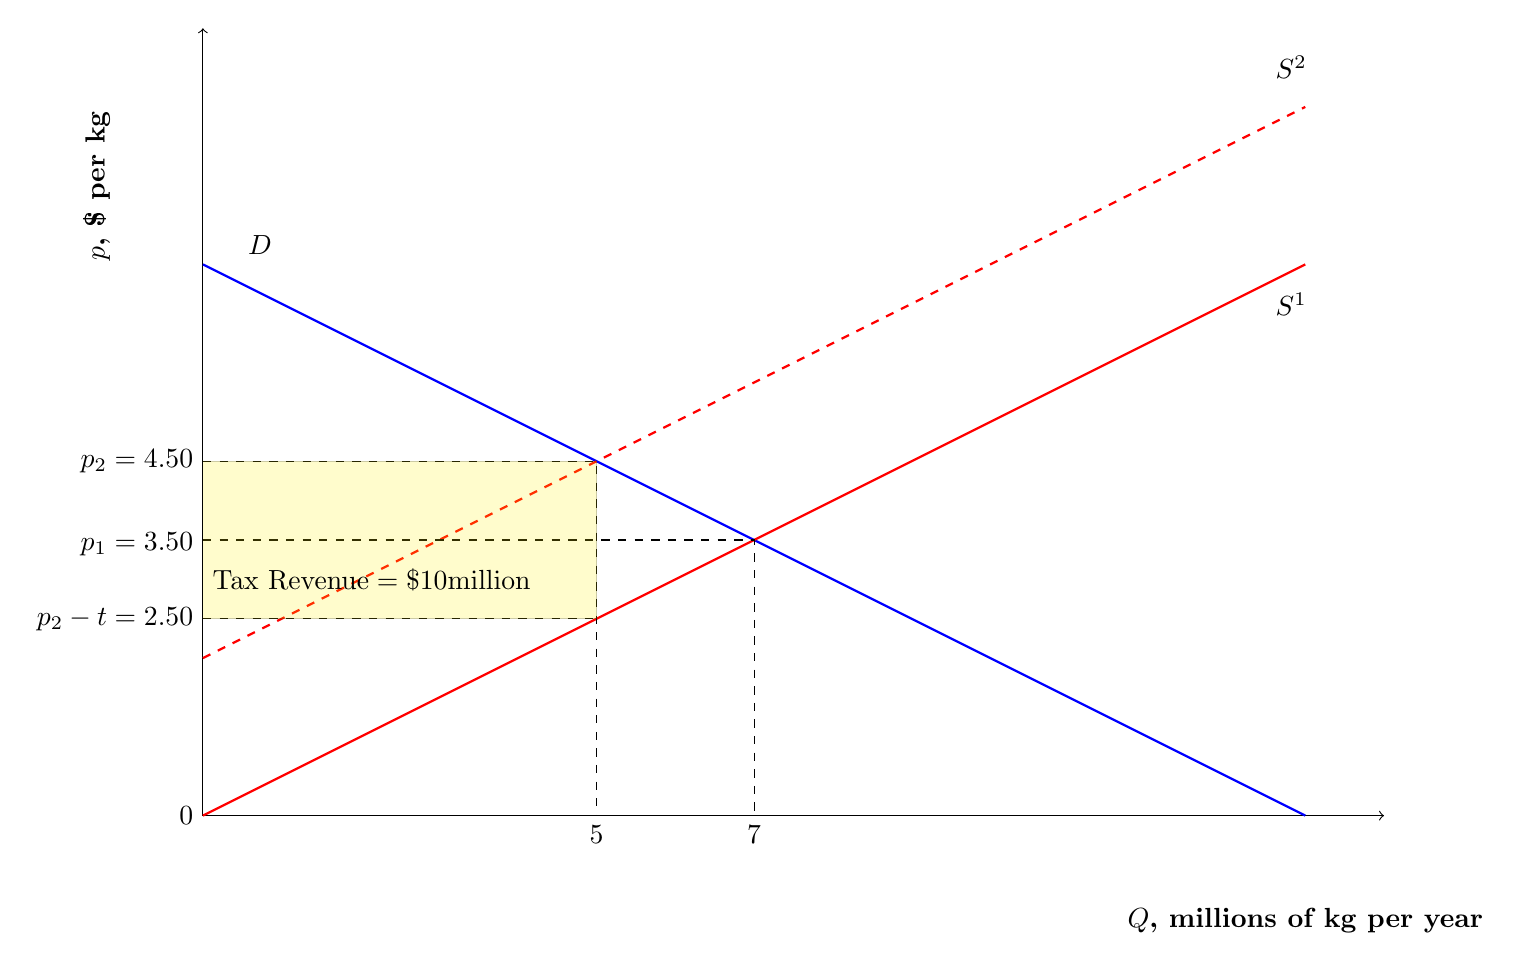
\begin{tikzpicture}
	% Draw axes
	%Y
	\draw[->] (0,0) -- (0,10) ;
	\draw[] (0,8) -- node[rotate=90, above=30pt] {\textbf{$p$, \$ per kg}} (0,8);
	%X
	\draw[->] (0,0) -- (15,0);
	\draw[] (14,0) -- node[below=30pt] {\textbf{$Q$, millions of kg per year}} (14,0);

	% Plot demand curve:
	% Curve given by: Q = 13 - 2p + 0.1Y
	% Assume Y= 10
	% Inverse demand: p = 7-0.5*Q
	\draw[color=blue, thick, domain=0:14] plot (\x,{7-0.5*\x});
	\node at (1,7.25) [left] {$D$};

	% Plot supply curve:
	% Curve given by: Q = 1 + 2p - 0.5p_{y}
	% Assume p_{y}= 2
	% Inverse supply: p = 0.5*Q
	\draw[color=red, thick, domain=0:14] plot (\x,{0.5*\x});
	\node at (13.5,6.5) [right] {$S^{1}$};
	
	% Assume t=2
	% Inverse supply: p = 2 + 0.5*Q
	\draw[color=red, thick, dashed, domain=0:14] plot (\x,{2+0.5*\x});
	\node at (13.5,9.5) [right] {$S^{2}$};

	%Plot illustrative lines
	% Original Equilibrium
	\draw[dashed] (0,3.5) -- (7,3.5) -- (7,0);
	% New Equilibrium
	\draw[dashed] (0,4.5) -- (5,4.5) -- (5,0);
	\draw[dashed] (0,2.5) -- (5,2.5);
	
	\draw[fill=yellow, opacity=0.2]  (0,4.5) -- (5,4.5) -- (5,2.5) -- (0,2.5) -- cycle;
	\node at (0,3) [right] {{$\text{Tax Revenue} = \$ 10 \text{million}$}};

	%Add axes labels
	%Origin%
	\node at (0,0) [left] {{0}};
	%Y Axis
	\node at (0,3.45) [left] {{$p_{1}=3.50$}};
	\node at (0,4.5) [left] {{$p_{2}=4.50$}};
	\node at (0,2.5) [left] {{$p_{2}-t=2.50$}};
	%X Axis
	\node at (7,0) [below] {{7}};
	\node at (5,0) [below] {{5}};

\end{tikzpicture}
}
\caption{The effects of a \$2.00/kg tax on gasoline producers}
\end{figure}
}

\frame{
	\frametitle{2. Using the Model: Specific Tax}
	%	The demand for gasoline:
	
	\begin{figure}[t!]
	\center
	\resizebox{!}{.35\linewidth}{

	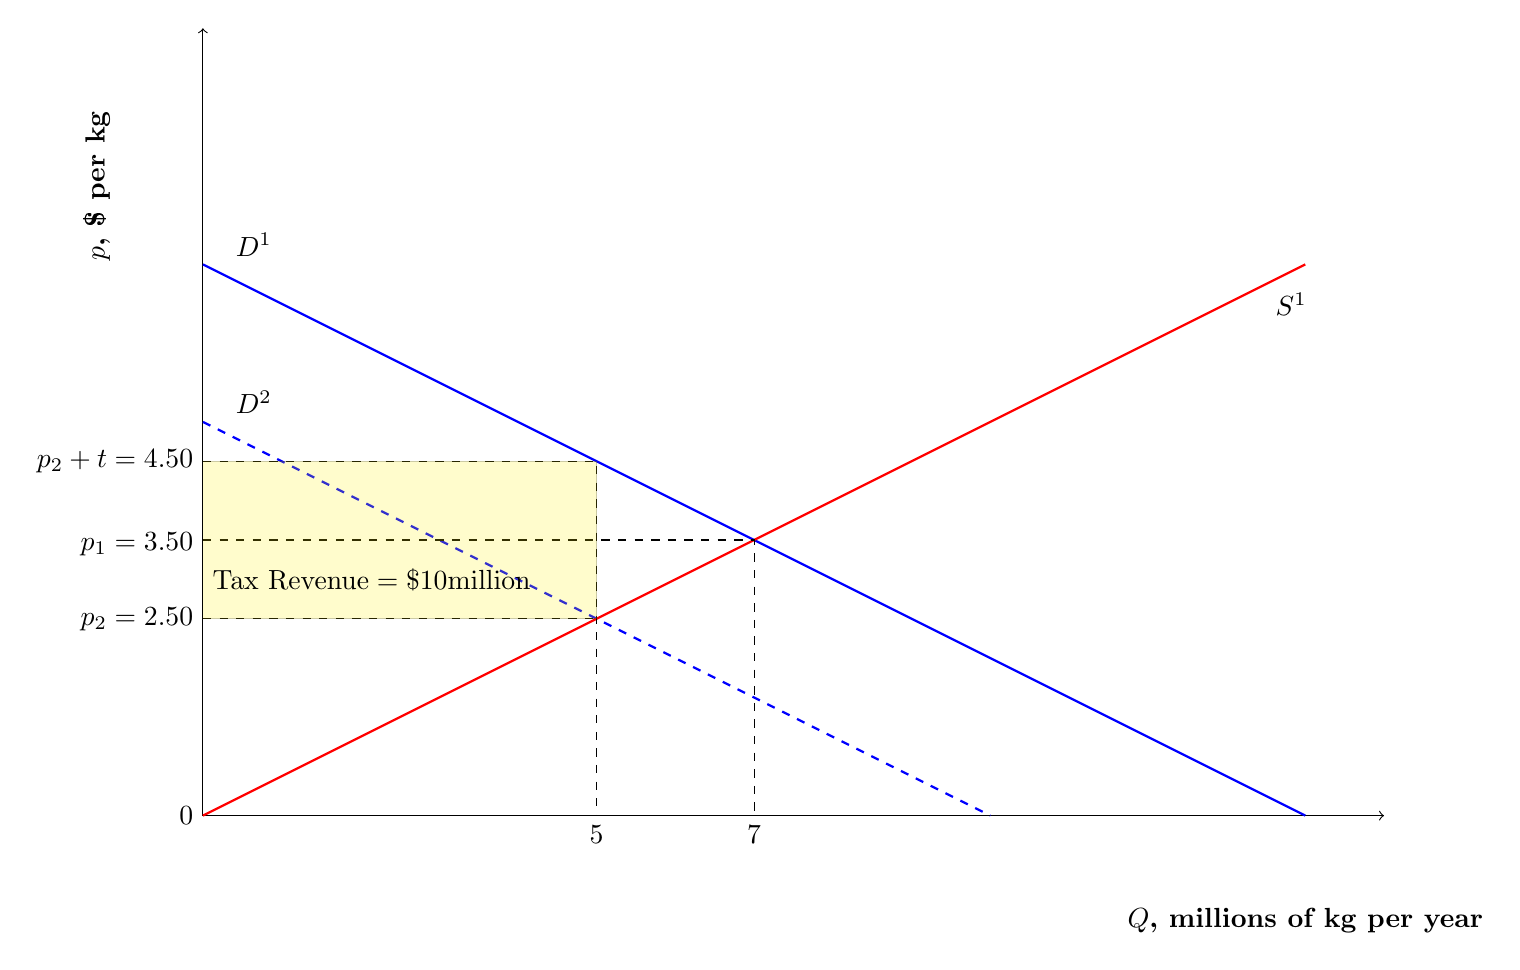
\begin{tikzpicture}
	% Draw axes
	%Y
	\draw[->] (0,0) -- (0,10) ;
	\draw[] (0,8) -- node[rotate=90, above=30pt] {\textbf{$p$, \$ per kg}} (0,8);
	%X
	\draw[->] (0,0) -- (15,0);
	\draw[] (14,0) -- node[below=30pt] {\textbf{$Q$, millions of kg per year}} (14,0);

	% Plot demand curve:
	% Curve given by: Q = 13 - 2p + 0.1Y
	% Assume Y= 10
	% Inverse demand: p = 7-0.5*Q
	\draw[color=blue, thick, domain=0:14] plot (\x,{7-0.5*\x});
	\node at (1,7.25) [left] {$D^{1}$};

	% Assume t = 2
	\draw[color=blue, thick, dashed, domain=0:10] plot (\x,{5-0.5*\x});
	\node at (1,5.25) [left] {$D^{2}$};

	% Plot supply curve:
	% Curve given by: Q = 1 + 2p - 0.5p_{y}
	% Assume p_{y}= 2
	% Inverse supply: p = 0.5*Q
	\draw[color=red, thick, domain=0:14] plot (\x,{0.5*\x});
	\node at (13.5,6.5) [right] {$S^{1}$};

	%Plot illustrative lines
	% Original Equilibrium
	\draw[dashed] (0,3.5) -- (7,3.5) -- (7,0);
	% New Equilibrium
	\draw[dashed] (0,4.5) -- (5,4.5) -- (5,0);
	\draw[dashed] (0,2.5) -- (5,2.5);
	
	\draw[fill=yellow, opacity=0.2]  (0,4.5) -- (5,4.5) -- (5,2.5) -- (0,2.5) -- cycle;
	\node at (0,3) [right] {{$\text{Tax Revenue} = \$ 10 \text{million}$}};

	%Add axes labels
	%Origin%
	\node at (0,0) [left] {{0}};
	%Y Axis
	\node at (0,3.45) [left] {{$p_{1}=3.50$}};
	\node at (0,4.5) [left] {{$p_{2}+t=4.50$}};
	\node at (0,2.5) [left] {{$p_{2}=2.50$}};
	%X Axis
	\node at (7,0) [below] {{7}};
	\node at (5,0) [below] {{5}};

\end{tikzpicture}
}
\caption{The effects of a \$2.00/kg tax on gasoline consumers}
\end{figure}
}

\frame{
	\frametitle{2. Using the Model: The Effects of A Specific Tax}
	\begin{itemize}
	\item Two key points:
		\begin{enumerate}
		\item As shown in the two figures, the imposition of specific sales tax yields the same
equilibrium regardless of \textit{who pays the tax}.
		\item[]
		\item The figures also show that the tax need not be fully passed on to consumers.
			\begin{itemize}
			\item Producers may bear some of the effects of a tax.
			\item What determines the extent of pass-through?
			\end{itemize}
		\end{enumerate}
	\end{itemize}
}

\frame{
	\frametitle{Outline}
	\begin{enumerate}
%	\item Big Government Gasoline
%	\item[]
	\item The Supply-and-Demand Model
		\begin{itemize}
		\item Demand
		\item Supply
		\item Market Equilibrium
		\end{itemize}
	\item[]
	\item Using the Model
		\begin{itemize}
		\item Changing fundamentals.
		\item The effects of government intervention.
		\end{itemize}
	\item[]
	\item \alert{Applying the model in practice.}
		\begin{itemize}
		\item When it works.
		\item When if fails.
		\end{itemize}
	\end{enumerate}
}

\section{Supply and Demand in Practice}

\frame{
	\frametitle{3. Applying the Model in Practice}
	\begin{itemize}
	\item The supply-and-demand model is a simple, but powerful tool for understanding how markets
will change in the future in response to shocks and changes in government policy.
		\begin{itemize}
		\item e.g. Dr. Copper, Mars Corp.
		\end{itemize}
	\item[]
	\item Unleashing the power of the model requires a deep understanding of the factors that will
affect demand and supply.
		\begin{itemize}
		\item Need to understand determinants of demand and supply/possible government actions.
		\end{itemize}
	\item[]
	\item We also need to know when the model is appropriate to use.
	\end{itemize}
}

\frame{
	\frametitle{3. Applying the Model in Practice}
	\begin{itemize}
	\item The supply-and-demand model works well as a tool for understanding markets that are
\textit{perfectly competitive}.
	\item[]
	\item Five characteristics of a perfectly competitive market:	
		\begin{enumerate}
		\item Many small buyers and sellers.
		\item Consumers believe all firms produce identical products.
		\item All market participants have full information about price and product
characteristics.
		\item Transaction costs (expenses over and above the price) are negligible.
		\item Firms can easily enter and exit the market, so competition is high.
		\end{enumerate}
	\item[]
	\item The model does not work well in non-competitive markets where there are a few sellers that
are price setters.
		\begin{itemize}
		\item For these markets, we need a different model.
		\end{itemize}
	\end{itemize}
}

\frame{
	\frametitle{3. Applying the Model in Practice}
	\begin{itemize}
	\item In practice, no market necessarily meets all five criteria.
	\item[]
	\item Still, the model is useful if the market is ``competitive enough''.
	\item[]
	\item What are some markets for which the model would work well?
	\end{itemize}
}

\frame{
	\frametitle{Supply and Demand: Takeaways}
	\begin{enumerate}
	\item The supply-and-demand model is a simple and powerful tool for understanding many markets.
	\item Model relates the quantity consumers demand and the quantity producers supply to own prices
and other factors.
	\item Using the model requires understanding how factors other than own price may shift demand
and supply, and how government intervention may affect prices in the market.
	\item The model works well for understanding markets that are competitive enough.
	\end{enumerate}
}

\end{document}
